\documentclass{article}
\usepackage{amsmath,graphicx,amsfonts,amssymb,amsthm,hyperref,amscd}


\title{Blake Notes}
\date{}
\author{Blake}
\begin{document}
\maketitle 


Sites:
\begin{enumerate}
  \item 
\end{enumerate} 



\section{Extracted Data}

\subsection{•}
 
The distribution of space debris was extracted using Web Plot Digitizer \cite{webPlotDigitizer} from NASA's collected data (See Figure \ref{fig:LEO_Debris_Distribution} \cite{NasaLEODensity}).

\begin{figure}[h]
	\centering
    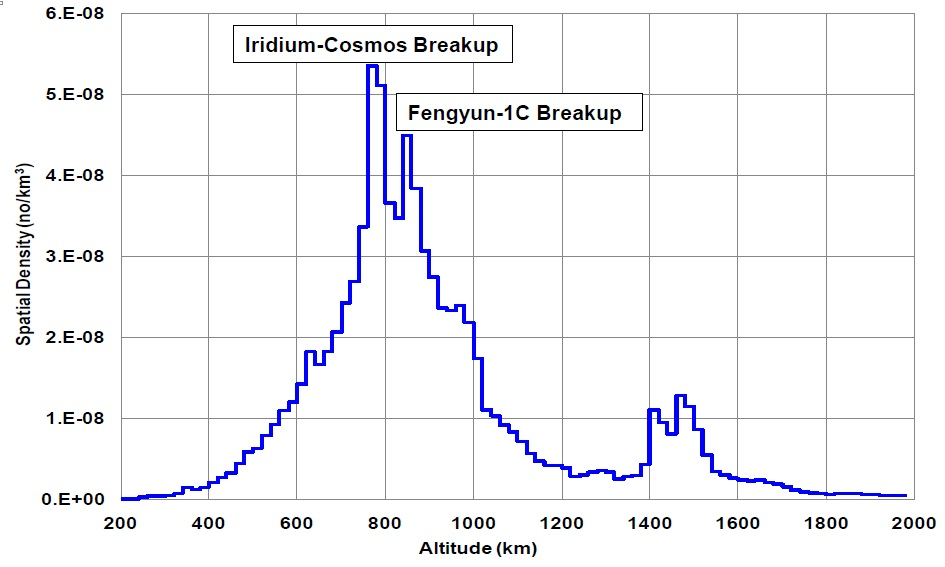
\includegraphics[width=0.75\textwidth]{figures/DebrisDensity.jpg}		
    \caption{The LEO debris distribution is primarily clustered in altitude corresponding to the Iridium-Cosmos Breakup and Fengyun-1C Breakup}
    \label{fig:LEO_Debris_Distribution}
\end{figure}


\section{Lasers}
\subsection{ORION}\cite{ORION}

\begin{itemize}
\item Ground based removal is feasible and testable
\item Cost
\begin{itemize}
\item A: remove ~ (30,000 debris objects) in 2 yrs full operation up to 800km altituded (20 hr/day) -> \$93M-\$108M
\item B: remove ~ (115,000 debris objects) in 3 yrs full operation up to 1500km altituded (20 hr/day) -> \$140M-\$176M
\end{itemize}

\end{itemize}


\subsection{SpacedBasedLaserSweep}\cite{SpaceBasedLaserSweep}
\begin{itemize}
\item  "the debris density at the most critical
altitude can be reduced by 23% with one laser in 10 years.
The laser will engage many objects at least two times, and
perform roughly 140,000 engagements in 10 years. This
means that the average time between two firings will be
between 30 min and 40 min."
\item "The simulated baseline mission has a duration of 10
years, a laser operating range of 20 km, a laser pulse
energy of 372 J and a beam tracking velocity limit of 151=s."
\end{itemize}

\subsection{PhippsSpaceLaserNudge}\cite{PhippsSpaceLaserNudge}


The mass and cost evaluations have been done by Photonic Associates, LLC 
\begin{itemize}
\item lasers used for LEO perturbing and GEO nudging
\item LEO NUDGE mass 5000kg, range = 1600km, \$220M, tagets 1 mass 1000kg
\item LEO small mass 6000kg, range = 250km, \$207M, tagets 10\^5 mass 0.05kg
\end{itemize}

\subsection{NumericalGroundBasedLasers}\cite{NumericalGroundBasedLasers}

\begin{itemize}
\item cost \$20/g to send objects to space
-implies ~2 times cost to send to space
\end{itemize}

\subsection{clearing with lasers}
-http://spie.org/newsroom/technical-articles-archive/4076-clearing-space-debris-with-lasers

"Energy costs 3¢/MJ on the ground, but any system designed to fly up and grapple or attach something to debris costs \$10,000/kg to place in orbit."


\subsection{PhippsSpaceLaserNow}\cite{PhippsSpaceLaserNow}

\begin{itemize}
\item Ground small -- target mass 0.75kg, 12k\$/debris, 16k\$/kg removed, 20,000 debris/yr, 200s/target

\item Ground large -- target mass 750kg, 4.7M\$/debris, 6.3k\$/kg removed, 750 debris/yr, 3.7yr/target

\item Polar ground large -- target mass 1400 kg, 5.3M\$/debris, 3.8k\$/kg removed, 300 debris/yr, 66 days/target
 
\item Space small -- target mass <0.038kg, 310\$/debris, 8\$/kg removed, 100k/4.6 30 debris/hr
20+=75km
\item Space Large -- target mass 1000kg, 280k\$/debris, 280\$/kg removed, 2k debris/4yr
600+-300km

\end{itemize}


\subsection{Summary}

The cost and reduction functions for any laser based LEO debris reduction method is dependent upon many attributes of the laser. An initial cost and reduction analysis would be to compare energy usage of the laser, energy needed to remove a single debris target, and the time taken to complete this task. While this would work provide a rough estimate, much more sophisticated cost and reduction analysis has already been computed at Photonic Associates LLC, taking into account numerous factors, such as mirror sizes, target size/mass, laser range, laser down time, laser tracking time, among others. The results are compiled below in Table \ref{table:Lasers}.
 
\begin{table}[h]
\centering
\begin{tabular}{||p{2cm}|c|c|c|c|c|c||} \hline
 Removal Rate (debris/yr) & Cost Rate (\$/yr) & Target Range (km) & Target Mass (kg) & Operation (perc) & G/S & Source \\ %[0.5ex] 
 \hline\hline
 15,000 & 93M - 108M & 800 & small & 83 & G & \cite{ORION} \\
 38,333 & 140M - 176M & 1500 & small & 83 & G & \cite{ORION} \\
 20,000 & 240M & 1000 & 0.75 & 80 & G & \cite{PhippsSpaceLaserNow} \\ 
 202 & 953M & 800 & 750 & 80 & G & \cite{PhippsSpaceLaserNow} \\
 75 & 397M & 800 & 1400 & 20 & G & \cite{PhippsSpaceLaserNow} \\
 
 260,000 & 80M & 760 & 0.083 & 50 & S & \cite{PhippsSpaceLaserNow} \\
 500 & 140M & 600 & 1000 & 100 & S & \cite{PhippsSpaceLaserNow} \\
 
% [1ex] 
 \hline
\end{tabular}
\caption{Compares different laser models}
\label{table:Lasers}
\end{table}



\section{Current Evaluation}
\subsection{CurrentCostRisk}\cite{CurrentCostRisk}
TODO

\subsection{Space Debris Assessing Risk and Responsibility}

TODO

\clearpage

\bibliographystyle{unsrt}
\bibliography{BlakeNotes}

\end{document}




